%\beginsupplement
\section{Supplementary Data}
\label{supplinfo}


\subsection{Potentials}
isoPAHAP tables?
curPAHIP tables?

The atomic coordinates and charges of the minimised 2pent15ring monomer.
Probably should also include the same for corannulene (can pull from CST paper).

\subsection{Dimer energy plots - isoPAHAP potential}

\subsection{Position restraint neglibigility at low temperature}

\subsection{Simulation length equilibration check}
Energies and radial distances don't change significantly when comparing eqm result from 3ns simulation (final 1ns) or 1ns simulation (final 500ps)
Percent error of intermolecular energies are less than 0.2\%
Percent error of radial distances are less than 3.5\%



\subsection{Corannulene crystal structure}
In order to assess / benchmark the structural metrics used in this paper, they have been applied to the known crystal structure of a corannulene. %Further comparison is made with a 2pent15ring system and published large cPAH systems - Actually this should be included in the discussion sections of the paper I think.

X-ray analysis of corannulene was conducted in 1975, and it was determined that the compound crystallises in space group \textit{P}$2_{1}/c$ \cite{hanson1976crystal}.

A crystal structure containing 18 molecules, taken from The Cambridge Crystallographic Data Centre \cite{CORANN11unitcell}, provides an independent verification of the analysis used in this work as well as a known experimental structure useful for comparison.  The crystal density and intermolecular distances are provided in Table \ref{table:crystal}.  Figure XX shows the crystal structure and alignment angles.

% Please add the following required packages to your document preamble:
% \usepackage{multirow}
\begin{table}[]
\centering
\caption{Molecular configuration metrics of corannulene crystal structure (collected from \cite{CORANN11unitcell}).}
\label{table:crystal}
\begin{tabular}{cc|cll}
\multicolumn{2}{c}{Density (kg/m3)} & 1.36 \cite{CORANN11unitcell}&  &  \\ \cline{1-3}
\multirow{3}{*}{Average intermolecular distance (nm)} & 1 molecule & 0.57 &  &  \\
 & 2 molecule & 0.72 &  &  \\
 & 3 molecule & 0.76 &  &  \\ \cline{1-3}
\multirow{3}{*}{Intermolecular distances (nm)} & 1 molecule & 0.55 x 10, 0.61 x 6 &  &  \\
 & 2 molecules & 0.61 x 2, 0.72 x 10, 0.73 x 2, 0.76 x 2, 0.78 x 2 &  &  \\
 & 3 molecules & 0.72 x 2, 0.73 x 4, 0.76 x 8, 0.78 x 2, 0.82 x 2 &  & 
\end{tabular}
\end{table}
%
%(using cut-off value of $R = 0.7$ nm)
%Intermolecular distances: 0.55 nm x 10, 0.61 nm x 6 (for first molecule); 0.61 x 2, 0.72 x 10, 0.73 x 2, 0.76 x 2, 0.78 x 2 (for second molecule), 0.72 x 2, 0.73 x 4, 0.76 x 8, 0.78 x 2, 0.82 x 2 (third molecule)... NOT SURE HOW TO SHOW THESE -> FOLLOW SAME PATTERN USED IN HOW I DISCUSS THIS IN THE PAPER (AVERAGE INTERMOLECULAR DISTS? - WOULD BE 0.57 NM FOR FIRST MOLECULE, ETC)
%
\begin{figure}[!tbh]
\centering
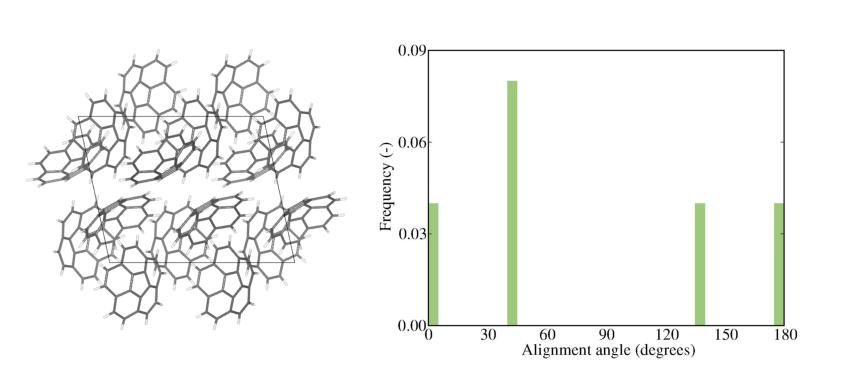
\includegraphics[width=0.65\linewidth]{Figures/corannulene_crystal.eps}
\caption{Snapshot of corannulene crystal structure (left) with alignment angle distribution (right).}
\label{fig:corannulene_crystal}
\end{figure}
%

\subsection{Cut-off distance sensitivities}
The selection of the cut-off distance, $R$, influences the calculated average intermolecular distances, coordination numbers, and alignment angles.

Due to the molecular arrangements of the homogeneous corannulene clusters (that is, sandwich-type stacking is not present), these results are the most sensitive to the selection of $R$.

- Include figure of CN histograms with r=0.5 for corannulene and 2pent15ring

- Include figures of alignment angles using R=0.5, 0.6, 0.7, 0.8 for a representative system (ann\_25?)

Note that for all systems, no neighbouring molecules are found using a cut-off distance of 0.400 nm or smaller.

\newpage